\documentclass[11pt]{standalone}
\usepackage[usenames]{color} %used for font color
\usepackage{amssymb} %maths
\usepackage{amsmath} %maths
\usepackage[no-math]{fontspec}
\usepackage{unicode-math}
\usepackage{libertinus}

\usepackage{pgf,xcolor}
\definecolor{itwm_blue}{HTML}{005A94}
\definecolor{itwm_red}{HTML}{C00000}
\usepackage{tikz}
\usepackage{pgfplots}
\pgfplotsset{compat=newest}

\begin{document}
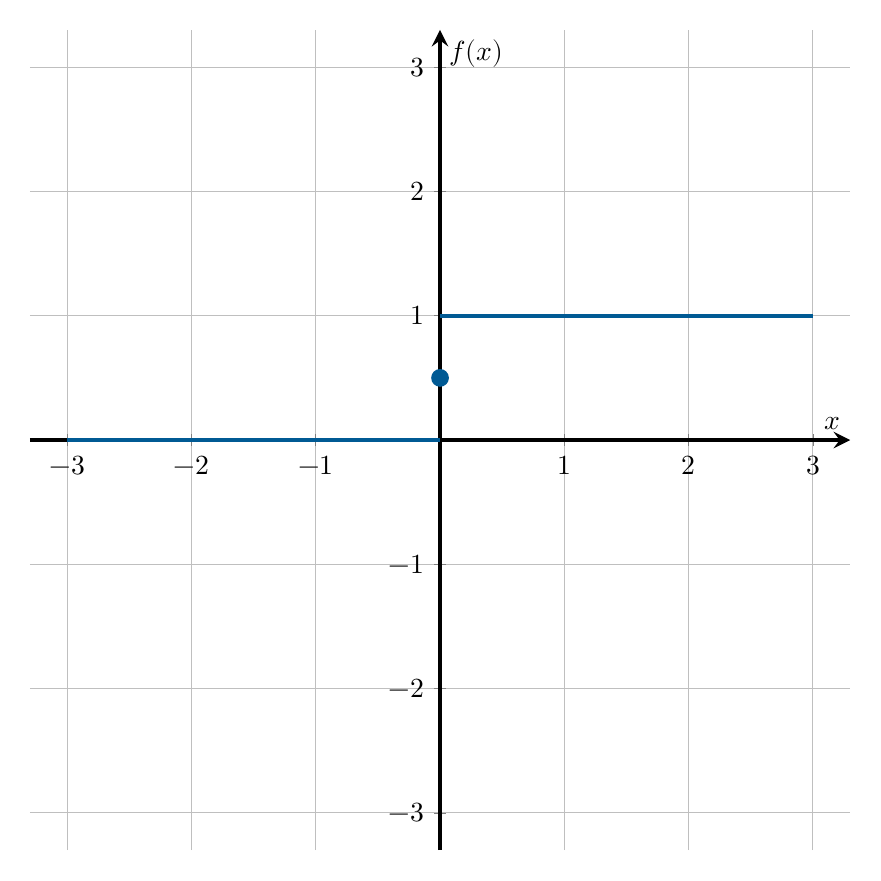
\begin{tikzpicture}
\begin{axis}[
    domain=-3:3,
    axis lines = center,
    xlabel = {$x$},
    ylabel = {$f(x)$},
    height=12cm, width=12cm, 
    grid = both,
    axis equal,
    axis line style={ultra thick},
    xmin=-3, xmax=3,
    ymin=-3*1.1, ymax=3*1.1,
]
    
% Teil 1: x < 0
\addplot[draw=itwm_blue, ultra thick, domain=-3:0] {0};
% Teil 2: x > 0  
\addplot[draw=itwm_blue, ultra thick, domain=0:3] {1};
% Punkt bei x=0
\addplot[only marks, mark=*, mark size=3pt, color=itwm_blue] coordinates {(0,0.5)};

\end{axis}
\end{tikzpicture}
\end{document}